\chapter{One Dimensional Fermi System}

\begin{figure}
	\centering
	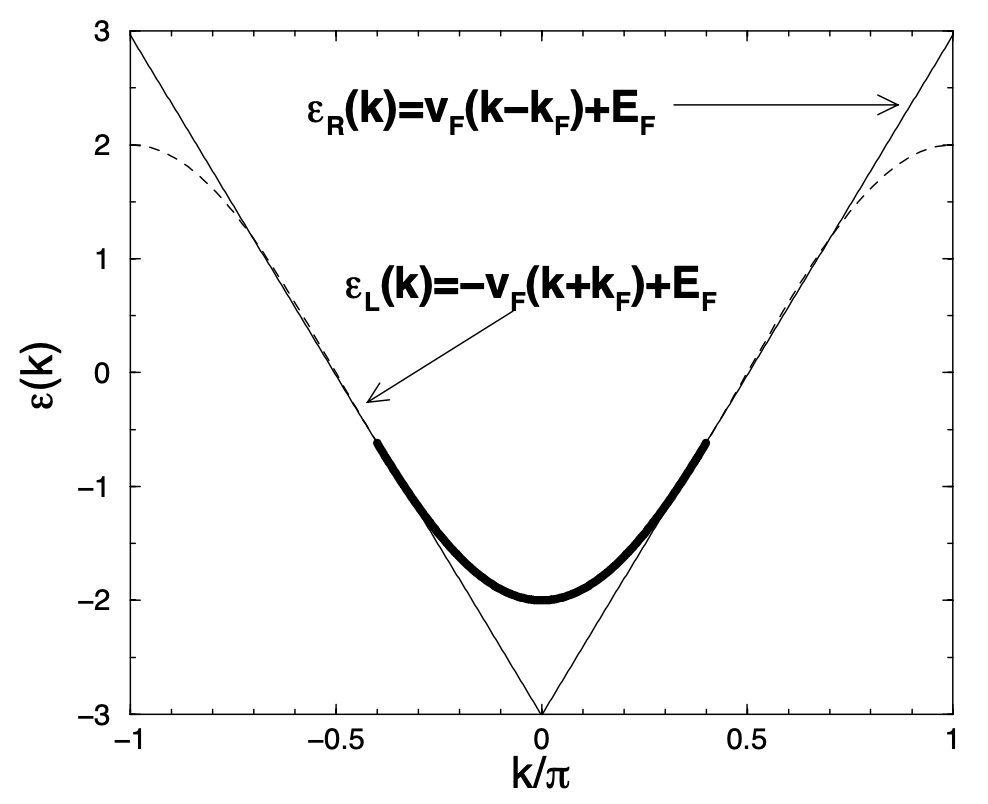
\includegraphics[width=0.4\linewidth]{pics/FL-linearize.png}
	\caption{Linearized Model.}
	\label{fig:bs-linearize}
\end{figure}

In this section, we discuss the one-dimensional interacting Fermi system, described by the Hamiltonian
\begin{equation}
	H = -\frac{1}{2}\sum_{i} (c_i^\dagger c_{i+1} + c_{i+1}^\dagger c_i) + \mu\sum_i c_i^\dagger c_i + \sum_{i,j,k,l} u_{ijkl} c_i^\dagger c_j^\dagger c_k c_l.
\end{equation}
The dispersion for the free theory is $\varepsilon(k) = -\cos k$, near the Fermi surface with momentum $k_F$, the spectrum can be approximately linearized (as shown in Fig.~\ref{fig:bs-linearize}), with the left and right moving fermion modes:
\begin{equation}
	\varepsilon_{R/L}(k) = \begin{cases}
		v_F (k - k_F) & r=R \\
		-v_F (k + k_F) & r=L
	\end{cases},\quad v_F = \sin k_F.
\end{equation}
The fermi momentum is (assume $N_L=N_R$)
\begin{equation}
	k_F = \frac{\pi N}{2L}.
\end{equation}
The state while all fermion modes filled below the Fermi surface and all modes empty above the Fermi surface is defined as the vacuum state $|0\rangle_0$.



\section{Field Theory for Luttinger Liquid}

In this section, we gives a field theoretical analysis of the interacting fermion system in 1D.
For the notational simplicity, we shift the momentum so that
\begin{equation}
	k \rightarrow k' = \begin{cases}
		k - k_F & r=R \\
		-k - k_F & r=L
	\end{cases}.
\end{equation}
The dispersion is then $\varepsilon_r(k) = v_F k$.
In this way, two Fermi points are brought to the origin, the left and right moving branches have the same dispersion.
The integral over momentum shell for both species of fermion can then be denoted by
\begin{equation}
	\int^\Lambda \frac{dK}{2\pi} \equiv \int_{-\Lambda}^\Lambda \frac{dk_L}{2\pi} + \int_{-\Lambda}^\Lambda \frac{dk_R}{2\pi}.
\end{equation}



\subsection{Effective Field Theory}

The effective field theory for the free field is
\begin{equation}
	Z_0 = \prod_{r=L/R}\int D\left[\bar\psi_r(k,\omega),\psi_r(k,\omega)\right] e^{-S_0},
\end{equation}
where the free field action is
\begin{equation}
	S_0 = \sum_{r=L/R} \int^\Lambda_{-\Lambda} \frac{dk}{2\pi} \int^\infty_{-\infty} \frac{d\omega}{2\pi} 
	\bar\psi_r(k,\omega)[-i\omega + v_F k]\psi_r(k,\omega),
\end{equation}
which gives the free field propagator:
\begin{equation}
	G_r(k,\omega) = -\langle \psi_r(k,\omega)\bar\psi_r(k,\omega)\rangle 
	= \frac{1}{i\omega - v_F k}.
\end{equation}
We then consider the rescaling of the cut-off $\Lambda \rightarrow \Lambda/s$. 
To make the free action scale invariant, we define the rescaled variables:
\begin{equation}
	k' = sk, \quad \omega' = s\omega, \quad 
	\psi'_r(k',\omega') = s^{-3/2}\psi_r(k,\omega).
\end{equation}
Then we consider the perturbation from quadratic and quartic terms:
\begin{equation}
\begin{aligned}
	\delta S_2 &= \sum_{r=L/R} \int^\Lambda_{-\Lambda}\frac{dk}{2\pi}\int^\infty_{-\infty} \frac{d\omega}{2\pi} 
	\mu(k,\omega) \bar\psi_r(k,\omega) \psi_r(k,\omega), \\
	\delta S_4 &= \frac{1}{2!2!} \int^\Lambda_{K,\omega} 
	u(4,3,2,1)\bar\psi(4)\bar\psi(3)\psi(2)\psi(1),
\end{aligned}
\end{equation}
where we have suppressed the momentum labels: 
\begin{equation}
	\psi(i) = \psi_{r_i}(k_i,\omega_i), \quad
	u(4,3,2,1) = u(K_4,\omega_4;K_3,\omega_3;K_2,\omega_2;K_1,\omega_1),
\end{equation}
and the integral is defined as:\footnote{The symbol $\bar\delta$ enforces momentum conservation mod $2\pi$, as is appropriate to any lattice problem. A process where lattice momentum is violated in multiples of $2\pi$ is called an \textit{umklapp process}.}
\begin{equation}
\begin{aligned}
	\int_{K \omega}^{\Lambda}
	=& \ \int^\Lambda \frac{d K_1 \cdots d K_4}{(2 \pi)^{4}} \int_{-\infty}^{\infty} \frac{d \omega_{1} \cdots d \omega_{4}}{(2 \pi)^{4}} \times 2 \pi \delta\left(\omega_{1}+\omega_{2}-\omega_{3}-\omega_{4}\right) \\
	&\ \times 2 \pi \bar{\delta}(K_1+K_2-K_3-K_4).
\end{aligned}
\end{equation}
Since this action separates into slow and fast pieces, the effect of mode elimination is simply to reduce $\Lambda$ to $\Lambda/s$ in the integral above. Rescaling moments and fields, we find that
\begin{equation}
	\mu'(k',\omega') = s\cdot\mu\left(\frac{k'}{s}, \frac{\omega}{s}\right).
\end{equation}
Expand $\mu$ in series:
\begin{equation}
	\mu(k, \omega)=\mu_{00}+\mu_{10} k+\mu_{01} i \omega+\cdots+\mu_{n m} k^{n}(i \omega)^{m}+\cdots,
\end{equation}
and compare both sides. The constant piece is a relevant perturbation.
This relevant flow reflects the readjustment of the Fermi sea to a change in chemical potential. 
The correct way to deal with this term is to include it in the free-field action by filling the Fermi sea to a point that takes $\mu_{00}$ into account. 
The next two terms are marginal and modify terms that are already present in the action.

We now turn on the quartic interaction, the dimensional analysis gives the transformation of $u$:
\begin{equation}
	u'_{i_4,i_3,i_2,i_1}(k'_i,\omega'_i) = u_{i_4,i_3,i_2,i_1}\left(\frac{k'_i}{s},\frac{\omega'_i}{s}\right).
\end{equation}
If we expand $u$ in a Taylor series in its arguments and compare coefficients, we find that the constant term u0 is marginal and the higher coefficients are irrelevant. 
Thus, $u$ depends only on its discrete labels and we can limit the problem to just a few coupling constants instead of the coupling function we started with. 
Furthermore, all reduce to just one coupling constant:
\begin{equation}
	u_0 = u_{LRLR} = u_{RLRL} = -u_{RLLR} = -u_{LRRL} \equiv u.
\end{equation}
Other couplings corresponding to the ($LL \rightarrow RR$) process are wiped out by the Pauli principle since they have no momentum dependence and cannot have the desired antisymmetry.

\subsection{RG at One-loop Level}

Consider the infinitesimal rescale $s=e^{dt}$. 
The one-loop contribution to the quadratic term is\footnote{We include an infinitesimal $e^{i\omega\eta}$ to ensure convergence as we do the integral over $\omega$ by closing the upper half-plane.}
\begin{equation}
	\mu^{(2)}_{LL} = 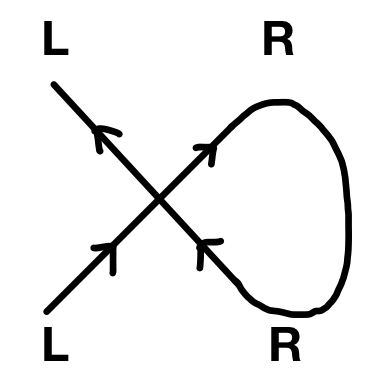
\includegraphics[align=c, width=0.125\linewidth]{pics/FL-1.png}
	= -u \int_{d\Lambda} \frac{dk}{2\pi}\int^\infty_{-\infty}\frac{d\omega}{2\pi}\frac{e^{i\omega \eta}}{i\omega - v_F k},
\end{equation}
where the integral on the momentum shell is
\begin{equation}
	\int_{d\Lambda}\frac{dk}{2\pi} = \int_{-\Lambda}^{-\Lambda(1-dt)} \frac{dk}{2\pi} + \int_{\Lambda(1-dt)}^{\Lambda} \frac{dk}{2\pi}.
\end{equation}
The result gives:
\begin{equation*}
	\mu^{(2)}_{LL}
	= -\frac{u\Lambda}{2 \pi}dt
\end{equation*}
By the symmetry $L \leftrightarrow R$, we know $\mu^{(2)}_{LL}=\mu^{(2)}_{RR}=\mu^{(2)}$, so the RG flow is
\begin{equation}
	\frac{d}{dt}\left[s\cdot\left(\mu+\mu^{(2)}\right)\right] = \mu - \frac{u\Lambda}{2\pi}.
\end{equation}
The one-loop correction to the quartic term ($u_{LRRL}=-u$) have two contributions.
One is called ZS' (zero sound) channel:\footnote{There is actually another zero sound channel ZS, but which has no contribution to the vertex because the diagram contains the vertex of the ($LL \rightarrow RR$) process, which has no relevant contribution the the vertex.}
\begin{equation}
\begin{aligned}
	u^{(2)}_{\mathrm{ZS'}} 
	&= 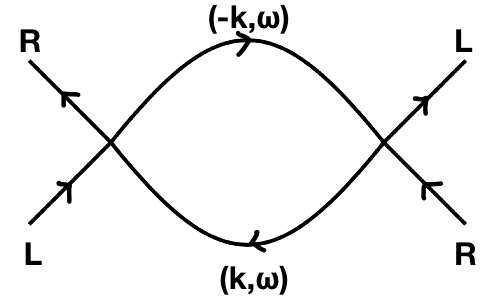
\includegraphics[align=c, width=0.2\linewidth]{pics/FL-2.png} \\
	&= -u^2 \int^\infty_{-\infty}\int_{\Lambda/s<|k|<\Lambda} \frac{d\omega dk}{(2\pi)^2} \frac{e^{i\omega\eta}}{(i\omega+v_F k)(i\omega-v_F k)} \\
	&= u^2\int_{\Lambda/s<|k|<\Lambda} \frac{dk}{2\pi} \frac{1}{2|k|} \\
	&= \frac{u^2}{2\pi}\frac{d\Lambda}{\Lambda}.
\end{aligned}
\end{equation}
The sign is obtained from contracting the Fermion field monomial:
\begin{equation*}
	\wick{
        \c1 {\bar\psi}_L \bar\psi_R \psi_L \c2 \psi_R
        \bar\psi_L \c2 {\bar\psi}_R \c1 {\psi}_L \psi_R
	} = -G_L G_R \bar\psi_R \psi_L \bar\psi_L \psi_R
	= -G_L G_R \bar\psi_L \bar\psi_R \psi_L \psi_R.
\end{equation*}
The other is called the BCS channel:\footnote{The $1/2$ factor comes from the symmetry factor of the diagram.}
\begin{equation}
	u^{(2)}_{\mathrm{BCS}} 
	= 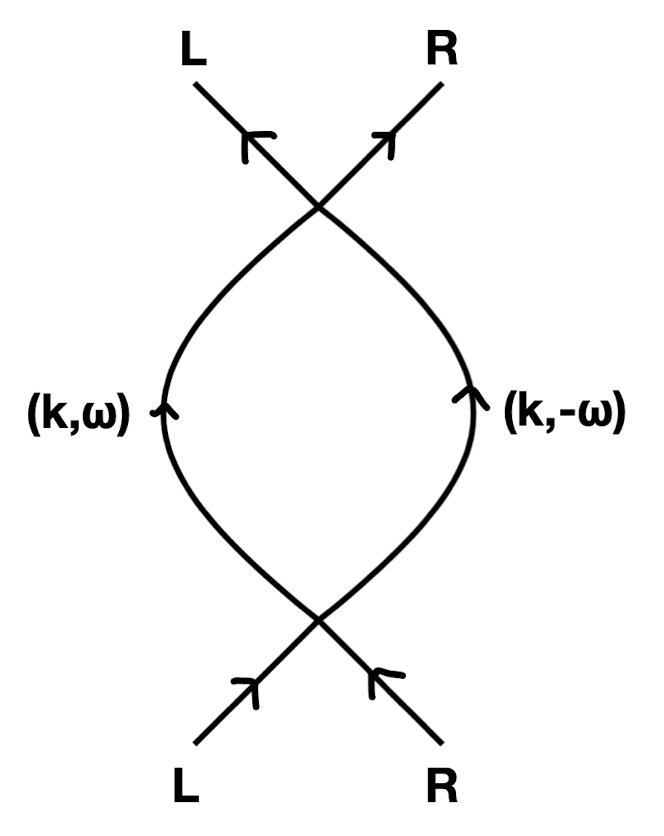
\includegraphics[align=c, width=0.15\linewidth]{pics/FL-3.png} 
	= -\frac{u^2}{2} \sum_{r=L/R}\int^\infty_{-\infty}\int_{d\Lambda} \frac{d\omega dk_i}{(2\pi)^2} \frac{e^{i\omega\eta}}{(i\omega-v_F k)(-i\omega-v_F k)}.
\end{equation}
The sign is obtained from the contraction:
\begin{equation*}
	\wick{
        \bar\psi_L \bar\psi_R \c1 \psi_L \c2 \psi_R
        \c1 {\bar\psi}_L \c2 {\bar\psi}_R \psi_L \psi_R
	} = -G_L G_R \bar\psi_L \bar\psi_R \psi_L \psi_R.
\end{equation*}
Note that we will obtained a factor of 2 since in this channel, the intermedia propagator can be left mover or right mover.
We see that two contributions cancel out:
\begin{equation}
	u^{(2)}_{\mathrm{ZS'}} + u^{(2)}_{\mathrm{BCS}} = 0.
\end{equation}
Together, the RG flow to the one-loop level is
\begin{equation}
	\frac{d\mu}{dt} = \mu - \frac{u\Lambda}{2\pi}, \quad
	\frac{du}{dt} = 0.
\end{equation}
The fixed point solution to the RG flow is:
\begin{equation}
	\mu^* = \frac{u^*\Lambda}{2\pi},
\end{equation}
where the fixed-point value of $u^*$ is arbitrary. 
The vanishing beta function predict that the ground state of one-dimensional weakly interacting Fermi gas remains gapless (rather than develops CDW order and becomes gapped).


\section{Bosonization}


In this section, we map the 1D interacting fermion system to a bosonic one.
From the RG analysis, we know that the low energy excitations are particle-hole modes:
\begin{equation}
	\rho_{k}^\dagger = \sum_{q} c_{q+k}^\dagger c_{q}, \quad
	\rho_{k} = \sum_{q} c_{q}^\dagger c_{q+k} = \rho_{-k}^\dagger.
\end{equation}

In the following, we restore the notation for the momentum (i.e., use the original momentum instead of the shifted one).
 

\subsection{Bosonic Hilbert Space}
To simplify the discussion, here we consider only a single branch of Fermion, as depicted in Fig.~\ref{fig:bs-hilbert}. The generalization to multiple branches is trivial since the dispersion is the same.

\begin{figure}
	\centering
	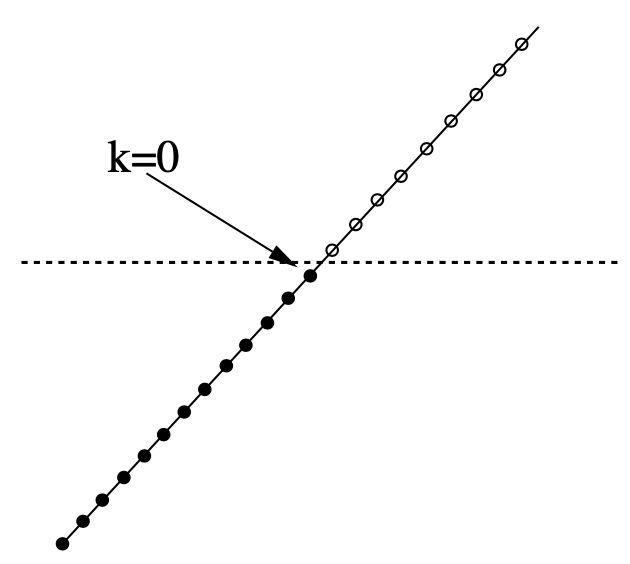
\includegraphics[width=0.25\linewidth]{pics/FL-hilbert.png}
	\caption{The vacuum state $|0\rangle_0$ of a single fermion branch.}
	\label{fig:bs-hilbert}
\end{figure}

The commutation relation between $\rho_k$ and $\rho_{k'}^\dagger$ is:\footnote{We use the identity $[AB,C] = A[B,C] + [A,C]B$ and $[A,BC]=\{A,B\}C - B\{A,C\}$.}
\begin{equation}
\begin{aligned}
	\left[\rho_{k}, \rho_{k'}^\dagger \right]
	&= \sum_{q_1, q_2} \left[c_{q_1}^\dagger c_{q_1+k}, c_{q_2+k'}^\dagger c_{q_2}\right] \\
	&= \sum_{q_1, q_2} \left\{c_{q_1}^\dagger \left[c_{q_1+k}, c_{q_2+k'}^\dagger c_{q_2}\right] +\left[c_{q_1}^\dagger, c_{q_2+k'}^\dagger c_{q_2}\right] c_{q_1+k}\right\} \\
	&= \sum_{q_1, q_2} \left\{ \delta_{q_1+k,q_2+k'} c_{q_1}^\dagger c_{q_2} -
		\delta_{q_1,q_2} c_{q_2+k'}^\dagger c_{q_1+k} \right\} \\
	&= \sum_{q}\left[c^\dagger_{q+k'-k} c_{q}-c^\dagger_{q+k'} c_{q+k}\right].
\end{aligned}
\end{equation}
For $k \ne k'$, it is clear that $[\rho_{k},\rho_{k'}^\dagger]=0$.
However, when $k = k'$, we should be careful about the subtraction, since it evolve two infinities of which the subtraction is ill-defined.

Here we deal with the infinity with the lattice regularization, i.e., we think of the linearized theory as the low-energy approximation of a lattice mode, where the dispersion form a single energy band.
The left/right movers are actually in a single band but with positive/negative momentum.
Consider for example the density operator for the right mover, the commutator of the right moving density operator is then
\begin{equation}
	\left[\rho_{k,r}, \rho_{k,r}^\dagger \right] = \sum_{0<q<\pi} [n_{q,r}-n_{k+q,r}].
\end{equation}

\begin{figure}
	\centering
	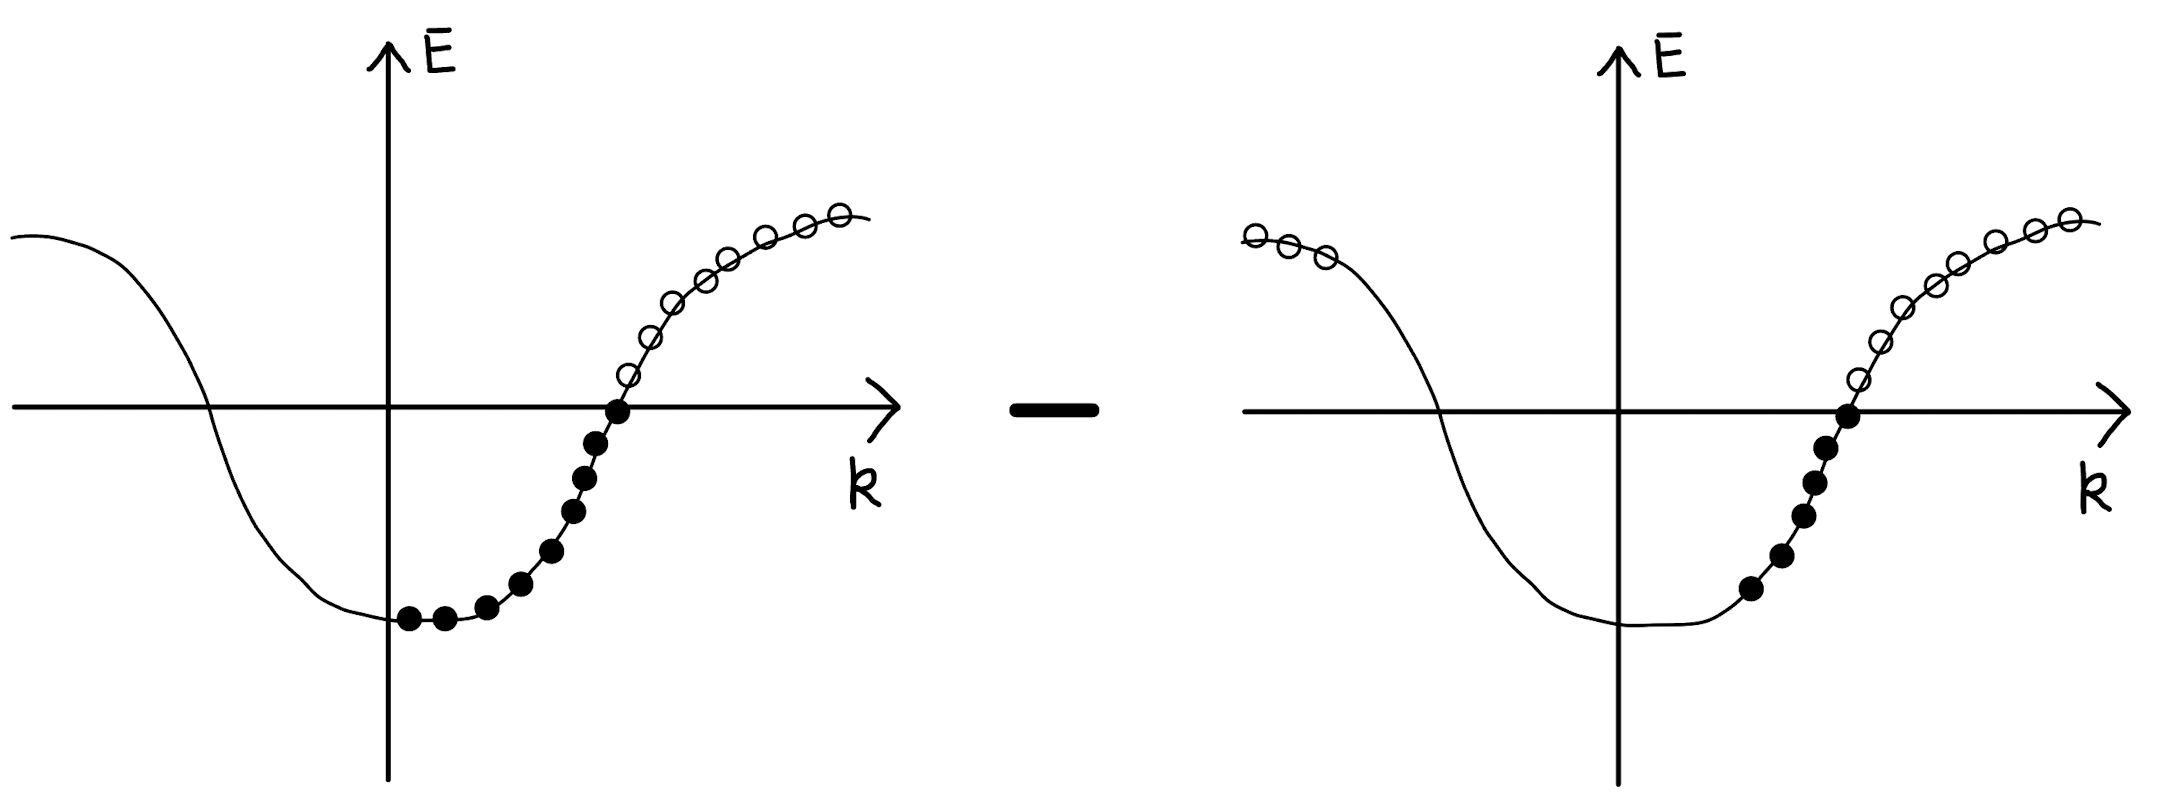
\includegraphics[width=0.6\linewidth]{pics/BS-k-shift}
	\caption{Shift of the right-moving modes.}
	\label{fig:bs-k-shift}
\end{figure}

Consider for example the case where $r=R,k>0$, as shown in Fig.~\ref{fig:bs-k-shift}.
The subtraction result in a sum of low-lying right-mover number operator minus a sum of high-energy left-mover number operator, which behaves like a constant in the low energy regime. 
The above analysis gives the commutation relation:
\begin{equation}
	\left[\rho_{k,r}, \rho_{kr}^\dagger \right] \simeq \frac{qL}{2\pi} \equiv n_q.
\end{equation}

\begin{framedrmk}[Normal Ordering]
Field theoretically, we can also evaluate the infinite subtraction by the normal-order expression:
\begin{equation}
	O = {:\mathrel{O}:} + \langle 0|O|0\rangle.
\end{equation}
For $k\ne k'$, since $\langle 0|c_k^\dagger c_k|0\rangle=0$, the normal ordering does not affect the result, while for the $k=k'$ case, the normal ordering takes care of the infinity of the particle number operator:
\begin{equation}
\begin{aligned}
	\sum_q [n_{q} - n_{q+k}]
	&= \sum_q \left[{:\mathrel{n_{q}}:} - {:\mathrel{n_{q+k}}:} 
		+ \langle0|n_{q}|0\rangle -\langle0|n_{q+k}|0\rangle \right] \\
	&= \sum_q [\langle0|n_{q}|0\rangle -\langle0|n_{q+k}|0\rangle].
\end{aligned}
\end{equation}
The final result gives the same result as the above discussions.
\end{framedrmk}

We denote the ground state with $N$ fermions as $|N\rangle_0$, which satisfies:
\begin{equation}
	\rho_{p>0}|N\rangle_0 = \rho^\dagger_{p<0}|N\rangle_0 = 0.
\end{equation}
We can thus define a set of canonical bosonic modes:
\begin{equation}
	b_p^\dagger = i\frac{\rho^\dagger_p}{\sqrt{n_p}}, \quad 
	b_p = -i\frac{\rho_p}{\sqrt{n_p}}, \quad [b_q,b_{q'}^\dagger] = \delta_{qq'}.
\end{equation}
We will assume $p>0$, and the $\pm i$ factor is a convention chosen for the future convenience.

Now we discuss the construction of the Hilbert space using the bosonic modes.
The $N$-particle sector is spanned by the states generated by applying $b_q^\dagger$'s to the ground state $|N\rangle_0$.
A general $N$-particle state has the form:
\begin{equation}
	|N\rangle = f(\{b_q^\dagger\})|N\rangle_0.
\end{equation}
Note that the bosonic mode $b_q$ does not change the particle number:\footnote{The particle number operator is defined by the normal order expression $\hat{N} = \sum_k {:\mathrel{c_{k}^\dagger c_{k}}:}$.}
\begin{equation}
	\left[\hat N, b_q \right] = \left[\hat N, b_q^\dagger \right] = 0.
\end{equation}
In order to construct the full Fock space, we also need to include a particle-number-changing operator, the \textit{Klein factor} $\hat F$, that shifts the total number of fermion by one, and commutes with bosonic operator $b_q$:
\begin{equation}
	\left[\hat F, b_q \right] = \left[\hat F, b_q^\dagger \right] = 0, \quad
	\left[\hat F, \hat N \right] = \hat F, \quad 
	\left[\hat F^\dagger, \hat N \right] = -\hat F^\dagger.
\end{equation}
For system with different fermion species (labeled by $\eta$), the set of operator
\begin{equation*}
	\{b_{q,\eta}, b_{q,\eta}^\dagger, \hat F_\eta, \hat N_\eta\}
\end{equation*}
form a complete operator basis for the Hilbert space within the low-energy regime.
However, note that the Klein factor also takes care of the fermionic statistics. 
That is, for the state denoted as
\begin{equation}
	|\{N_i\}\rangle = |N_1,N_2,\cdots,N_m\rangle
\end{equation}
The Klein factor $\hat F_\eta$ acting on the state will contribute an additional factor
\begin{equation}
	\hat F_\eta|\{N_i\}\rangle = \exp\left(i\pi\sum_{j=1}^{\eta-1}N_j\right)|N_1,\cdots,N_\eta-1,\cdots,N_m\rangle.
\end{equation}

\subsection{Bosonization of Fermion Field}
Now we try to express the fermion operator 
\begin{equation}
	\psi(x) = \frac{1}{\sqrt{L}} \sum_p e^{ipx} c_{p}
\end{equation}
by the bosonic operator set.
First we consider the commutation relation between the fermion field operator and bosonic mode:
\begin{equation}\label{eq:bs-comm-1}
\begin{aligned}
	\left[b_q,\psi(x)\right] &= \frac{1}{\sqrt L}\frac{i}{\sqrt{n_q}}\sum_{k}\sum_{p} e^{ipx} [c^\dagger_{k}c_{k+q,r'},c_{p}] \\
	&= -\frac{1}{\sqrt L} \frac{i}{\sqrt{n_q}} \sum_{p} e^{ipx} c_{p+q} 
	= -i\frac{1}{\sqrt{n_q}} e^{-iqx} \psi(x).
\end{aligned}
\end{equation}
Similarly,
\begin{equation}\label{eq:bs-comm-2}
	\left[b_q^\dagger,\psi(x)\right] = i\frac{e^{iqx}}{\sqrt{n_q}} \psi(x).
\end{equation}
For future convenience, we define a c-number factor:
\begin{equation}
	\alpha_q(x) \equiv \frac{1}{\sqrt{n_q}} e^{iqx},\quad
	[b_q^\dagger,\psi(x)] = i\alpha_q(x) \psi(x),\quad
	[b_q,\psi(x)] = -i \alpha^*_q(x) \psi(x).
\end{equation}
Since $b_q|N\rangle_0 = 0$, the commutation relation (\ref{eq:bs-comm-1}) leads to
\begin{equation}
	\left[b_{q}, \psi(x)\right]|N\rangle_{0} 
	=b_{q} \psi(x)|N\rangle_{0} 
	= -i\alpha_q^*(x) \psi(x)|N\rangle_{0}.
\end{equation}
Thus, $\psi(x)|N\rangle_0$ is an eigenstate of $b_q$, i.e., a coherent state:
\begin{equation}
	\psi(x)|N\rangle_0 
	= \Lambda(x) \hat F \exp\left[-i\sum_{q>0} \alpha_q^*(x) b_q^\dagger\right]|N\rangle_0
\end{equation}
where $\Lambda(x)$ is a c-number, which can be determined by
\begin{equation*}
	{}_{0}\langle N-1|\psi(x)| N\rangle_{0}=\Lambda(x)\ {}_{0}\langle N|\exp \left[-i\sum_{q>0} \alpha^*_q(x) b_{q}^{\dagger}\right]| N\rangle_{0} = \Lambda(x).
\end{equation*}
The left-hand side can be computed directly, the result is\footnote{Note that the Fermi point locates at $k_F=\frac{2\pi N}{L}$.}
\begin{equation}
	\Lambda(x) = \frac{1}{\sqrt L}\sum_k e^{ikx}\ {}_{0}\langle N-1| c_{k,r}|N\rangle_0 
	= \frac{1}{\sqrt L} e^{i\frac{2\pi N}{L}},
\end{equation}
In this way, we get
\begin{equation}
	\psi(x)|N\rangle_{0} = \frac{\hat F}{\sqrt{L}} e^{i \frac{2 \pi \hat{N} x}{L}} \exp \left[-i\sum_{q>0} \alpha^*_q(x) b_{q}^{\dagger}\right]|N\rangle_{0}
\end{equation}
The commutation relation (\ref{eq:bs-comm-2}) also leads to:\footnote{We denote $\alpha_q(x) \equiv e^{iqx}/\sqrt{n_q}$ to simplify the notation.}
\begin{equation*}
\begin{aligned}
	\psi(x) b_{q}^{\dagger} 
	&=\left[b_{q}^{\dagger}-i\alpha_{q}(x)\right] \psi(x) \\
	\Rightarrow \psi(x)\left(b_{q}^{\dagger}\right)^{n} 
	&=\left[b_{q}^{\dagger}-i\alpha_{q}(x)\right]^{n} \psi(x) \\
	\Rightarrow \psi(x) f\left[\left\{b_{q}^{\dagger}\right\}\right] 
	&=f\left[\left\{b_{q}^{\dagger}-i\alpha_{q}(x)\right\}\right] \psi(x).
\end{aligned}
\end{equation*}
Then, for a generic $N$-particle state:
\begin{equation}\label{eq:bs-temp1}
\begin{aligned}
	\psi(x)|N\rangle 
	&=f\left[\left\{b_{q}^{\dagger}-i\alpha_{q}(x)\right\}\right] \psi(x)|N\rangle_{0} \\
	&=f\left[\left\{b_{q}^{\dagger}-i\alpha_{q}(x)\right\}\right] \frac{\hat{F}}{\sqrt{L}} e^{i \frac{2 \pi \hat{N} x}{L}} \exp \left[-i\sum_{q>0} \alpha^*_{q}(x) b_{q}^{\dagger}\right]|N\rangle_{0} \\
	&=\frac{\hat{F}}{\sqrt{L}} e^{i \frac{2 \pi \hat{N} x}{L}} \exp \left[-i\sum_{q>0} \alpha^*_{q}(x) b_{q}^{\dagger}\right] f\left[\left\{b_{q}^{\dagger}-\alpha_{q}(x)\right\}\right]|N\rangle_{0}.
\end{aligned}
\end{equation}
Using the BCH formula
\begin{equation}
	e^A B e^{-A} = e^{[A,\cdot]} B = B + [A,B] + \frac{1}{2!}[A,[A,B]]+\cdots,
\end{equation}
we have the identity:
\begin{equation*}
\begin{aligned}
	\exp \left[-i\sum_{q>0} \alpha_{q}(x) b_{q}\right] b_{q}^{\dagger} \exp \left[i\sum_{q>0} \alpha_{q}(x) b_{q}\right] &=b_{q}^{\dagger}-i\alpha_{q}(x) \\
	\Rightarrow \exp \left[-i\sum_{q>0} \alpha_{q}(x) b_{q}\right] f\left[b_{q}^{\dagger}\right] \exp \left[i\sum_{q>0} \alpha_{q}(x) b_{q}\right] &=f\left[\left\{b_{q}^{\dagger}-i\alpha_{q}(x)\right\}\right].
\end{aligned}
\end{equation*}
Eq.~(\ref{eq:bs-temp1}) can be further simplified to:
\begin{equation*}
\begin{aligned}
	\psi(x)|N\rangle 
	=&\ \frac{\hat{F}}{\sqrt{L}} e^{i \frac{2 \pi \hat{N} x}{L}} e^{-i\sum_{q>0} \alpha^*_{q}(x) b_{q}^{\dagger}} e^{-i\sum_{q>0} \alpha_{q}(x) b_{q}} f\left[b_{q}^{\dagger}\right] e^{i\sum_{q>0} \alpha_{q}(x) b_{q}} |N\rangle_{0} \\
	=&\ \frac{\hat{F}}{\sqrt{L}} e^{i \frac{2 \pi \hat{N} x}{L}} \exp \left[-i\sum_{q>0} \alpha^*_{q}(x) b_{q}^{\dagger}\right] \exp \left[-i\sum_{q>0} \alpha_{q}(x) b_{q}\right]|N\rangle.
\end{aligned}
\end{equation*}
We thus express the Fermi field operator in bosonic operator:
\begin{equation}\label{eq:bs-fermi-field-1}
	\psi(x) = \frac{\hat{F}}{\sqrt{L}} e^{i \frac{2 \pi \hat{N} x}{L}} e^{-i\sqrt{2\pi}\varphi^\dagger(x)} e^{-i\sqrt{2\pi}\varphi(x)},
\end{equation}
where we have introduced a bosonic field:\footnote{The ``converging factor'' $e^{-a q / 2}$ is important in defining a proper bosonic theory in 1D. These equations should always be viewed as having $e^{-a q / 2}$ to ensure convergence at intermediate steps, but final results should be written taking $a \rightarrow 0^{+}$.}
\begin{equation}
	\varphi(x) = \frac{1}{\sqrt{2\pi}}\sum_{q>0} e^{-a q/2} a_{q}(x) b_{q}.
\end{equation}
Now we introducing the bosonic field:
\begin{equation}
	\phi(x) \equiv \varphi(x)+\varphi^{\dagger}(x)
	= \frac{1}{\sqrt{2\pi}} \sum_{q>0} \frac{e^{-a q/2}}{\sqrt{n_q}} \left[e^{i q x} b_{q}+e^{-i q x} b_{q}^{\dagger}\right].
\end{equation}
We can expressed the fermion field as:\footnote{We use the identity $e^A e^B = e^{A+B}e^{\frac{1}{2}[A,B]}$ if both $A$ and $B$ commutes with $[A,B]$.}
\begin{equation*}
	\psi(x) = \frac{\hat{F}}{\sqrt{L}} e^{i\frac{2\pi \hat N x}{L}} e^{-i\sqrt{2\pi}\phi(x)}
	e^{\pi[\varphi(x),\varphi^\dagger(x)]}.
\end{equation*}
The commutation relation between $\varphi$ and $\varphi^\dagger$ is
\begin{equation*}
	\left[\varphi(x),\varphi^\dagger(y)\right]
	= \frac{1}{L} \sum_q \frac{e^{iq(x-y+ia)}}{q} 
	= -\frac{1}{2\pi}\ln\left\{ 1-\exp\left[\frac{2\pi i}{L}(x-y+ia)\right]\right\}.
\end{equation*}
Set $x=y$, take limit $a\rightarrow 0^+$,
\begin{equation*}
	\exp\left\{\pi[\varphi(x),\varphi^\dagger(x)] \right\} = \lim_{a\rightarrow0^+} \left[1-\exp\left(-\frac{2\pi a}{L}\right)\right]^{-\frac{1}{2}}
	\rightarrow \sqrt{\frac{L}{2\pi a}}.
\end{equation*}
so we have
\begin{equation}\label{eq:bs-fermi-field}
	\psi(x) = \frac{\hat{F}}{\sqrt{2\pi a}}e^{i\frac{2\pi\hat N x}{L}}e^{-i\sqrt{2\pi}\phi(x)}.
\end{equation}
The divergent factor $1/\sqrt{2\pi a}$ appears because Eq.~(\ref{eq:bs-fermi-field}) is not normal-ordered.
We can check the result by normal-ordering the bilinear term $\psi^\dagger(x+a)\psi(x)$.
Insert Eq.~(\ref{eq:bs-fermi-field}) into the expression, we have:
\begin{equation}
	\psi^\dagger(x+a)\psi(x)
	\simeq \frac{e^{-i\frac{2\pi\hat N a}{L}}}{2\pi a}
	e^{i\sqrt{2\pi}\partial_x\phi(x)  a} 
	e^{\pi[\phi(x+ a),\phi(x)]}.
\end{equation}
The commutation relation is:
\begin{equation}
\begin{aligned}
	\left[\phi(x),\phi(y)\right] 
	&= -\frac{1}{2\pi}\ln \left\{\frac{1-\exp \left[\frac{2 \pi i}{L}(x-y+i  a)\right]}{1-\exp \left[-\frac{2 \pi i}{L}(x-y-i  a)\right]}\right\} \\
	&\stackrel{ a \rightarrow 0}{\longrightarrow} 
		\frac{i}{2} \operatorname{sgn}(x-y)-\frac{i}{L}(x-y).
\end{aligned}
\end{equation}
To the lowest order of $a/L$: 
\begin{equation}
	\psi^\dagger(x+a)\psi(x) \simeq \frac{i}{2\pi a} + \frac{\hat N+1}{L} - \frac{1}{\sqrt{2\pi}}\partial_x\phi(x).
\end{equation}
The normal ordering will delaminate all constant, including the divergent one:
\begin{equation}
	{:\mathrel{\psi^\dagger(x+a)\psi(x)}:}
	= \frac{\hat N}{L} - \frac{1}{\sqrt{2\pi}}\partial_x\phi(x).
\end{equation}
We will show in the following the above equation agrees with the bosonization of fermion bilinear $\psi^\dagger(x)\psi(x)$ term.




\subsection{Bosonization Dictionary}
Now we are going to establish a bosonization dictionary.
To tell the complete story, we are now working for both the right-moving and left-moving fermion branches.
In this case, we express the fermion as a spinor:
\begin{equation}
	\psi = \left(\begin{array}{c}
		\psi_L \\ \psi_R
	\end{array} \right),\quad
	\bar\psi = \psi^\dagger\sigma^x =  \left(\begin{array}{cc}
		\psi^\dagger_R & \psi_L^\dagger
	\end{array} \right).
\end{equation}
We also define a new set of bosonic fields
\begin{equation}
	\phi(x) \equiv \phi_R(x) + \phi_L(x), \quad
	\theta(x) \equiv \phi_R(x) - \phi_L(x).
\end{equation}
First we consider the fermion bilinear (for $r=L/R$):
\begin{equation}
\begin{aligned}
	{:\mathrel{\psi_r^\dagger(x)\psi_r(x)}:}
	&= \frac{1}{L}\sum_{q} {:\mathrel{c_{q,r}^\dagger c_{q,r}}:} + \frac{1}{L}\sum_{q>0}[e^{-iqx}\rho^\dagger_{q,r}+e^{iqx}\rho_{q,r}] \\
	&= \frac{\hat N_r}{L} - \frac{1}{2\pi} \sum_{q>0} \frac{iq}{\sqrt{n_q}} \left[e^{iqx}b_{q,r} - e^{-iqx}b^\dagger_{q,r}\right].
\end{aligned}
\end{equation}
We then get:
\begin{equation}
	{:\mathrel{\psi^\dagger(x)\psi(x)}:}
	= \frac{\hat N_L +\hat N_R}{L} - \frac{1}{\sqrt{2\pi}} \partial_x \left[\phi_L(x)+\phi_R(x)\right].
\end{equation}



Now we go back to the Hamiltonian with linear dispersion (for single fermion branch):
\begin{equation}
	H_0 = v_F \sum_{k,r} k\ {:\mathrel{c_{k,r}^\dagger c_{k,r}}:} 
	= v_F \int dx\ {:\mathrel{\psi^\dagger(x)(-i\partial_x)\psi(x)}:}.
\end{equation}
Since $b_q^\dagger$ raise the energy of any eigenstate of $H_0$ by $q$ unit, we have the commutation relation:
\begin{equation}
	\left[H_0,b_{q,r}^\dagger\right] = q b_{q,r}^\dagger.
\end{equation}
The Hamiltonian satisfies such relation can only be the bosonic bilinear:
\begin{equation}
	H_0 = v_F \sum_{r}\sum_{q>0} q b_{q,r}^\dagger b_{q,r} + \frac{\pi v_F}{L} \sum_r \hat{N}_r(\hat{N}_r+1).
\end{equation}
The constant part comes from the fact that
\begin{equation*}
	H_0|N\rangle_0 = \frac{2\pi v_F}{L} \frac{\sum_r\hat{N}_r(\hat{N}_r+1)}{2}|N\rangle_0, \quad
	b_{q,r}^\dagger b_{q,r} |N\rangle_0 = 0.
\end{equation*}
Also, the bosonic operator can also be expressed as
\begin{equation}
	H_0 = \frac{v_F}{2} \int dx\ {:\mathrel{[\partial_x \phi(x)]^2}:} + \frac{\pi v_F}{L}\sum_r \hat{N}_r(\hat{N}_r+1).
\end{equation}





